\chapter{OpenStack Folsom}\label{cap:openstack}
\noindent El presente cap\'itulo pretende describir, con cierto detalle, la implementaci\'on del framework para cloud IaaS elegida. Partiremos de una visi\'on global que se ir\'a concretando para describir las responsabilidades y relaciones entre cada parte del cloud.

\section{Arquitectura global}\label{sec:arquitecturaglobal}
\noindent La figura \ref{fig:arquitecturaos} muestra los tres los componentes operacionales b\'asicos de OpenStack Folsom:

\begin{description}
 \item[N\'ucleo funcional:] OpenStack Compute, OpenStack Quantum (Redes) y OpenStack Storage.
 \item[Interfaz web de control:] OpenStack Horizon Dashboard.
 \item[Servicios compartidos:] OpenStack Glance, OpenStack Keystone y otros servicios indirectos como la persistencia en base de datos o la cola de mensajes.
\end{description}

\begin{figure}[tbp]
\begin{center}
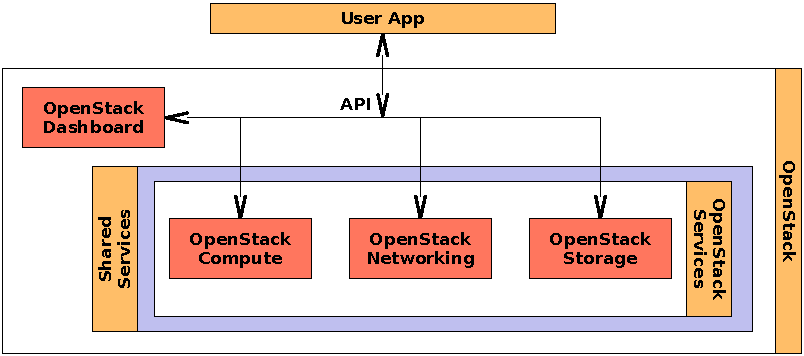
\includegraphics[width=0.9\textwidth]{imagenes/012.pdf}
 \caption{Arquitectura de alto nivel de OpenStack}
\label{fig:arquitecturaos}
\end{center}
\end{figure}


Los distintos componentes han sido ideados de manera que no se compartan estructuras globales de estado ---\emph{shared nothing}. Esto aporta al administrador del cloud la flexibilidad necesaria para poder repartir indiscriminadamente los m\'odulos constitutivos a lo largo de la infraestructura subyacente. De forma condensada, la figura \ref{fig:despliegueos} expone un ejemplo de despliegue posible de un cloud usando OpenStack Folsom. Apoy\'andonos en ella, resumiremos la funcionalidad que otorga cada m\'odulo de OpenStack, en rojo, junto con los servicios adicionales sobre los que se apoyan, en violeta. A pesar de que no se haya incluido en la figura por cuestiones de claridad, la comunicaci\'on inter-m\'odulo se realiza por paso de mensajes as\'incronos usando una cola. Las dos implementaciones de cola de mensajes documentadas son \texttt{RabbitMQ} y \texttt{Qpid}, siendo esta \'ultima la utilizada en el despliegue de prueba.

\begin{figure}[tbp]
\begin{center}
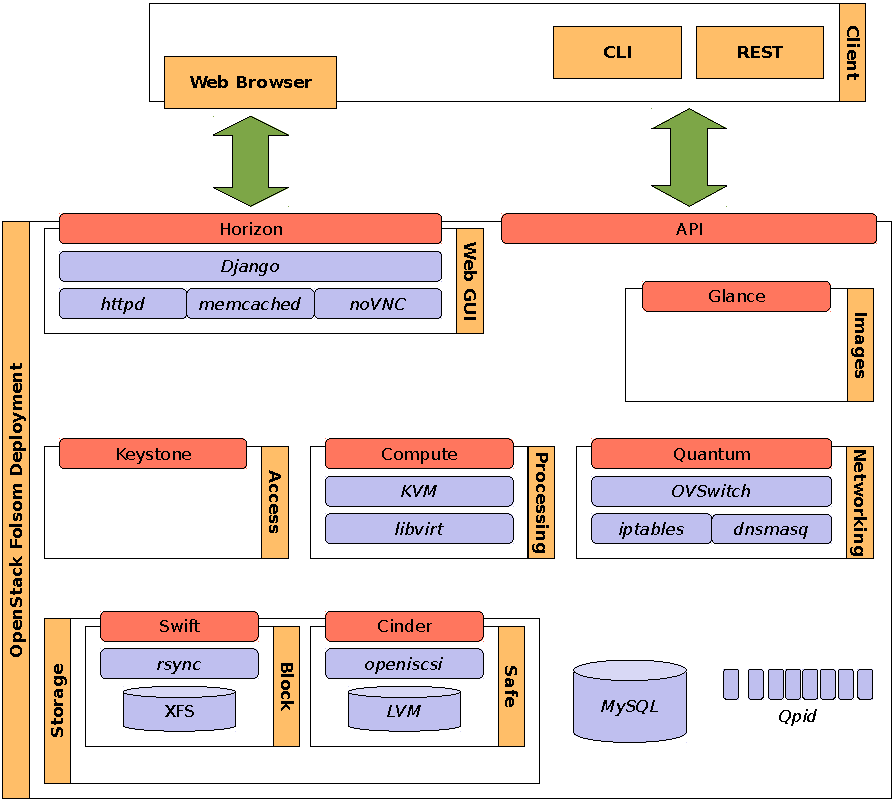
\includegraphics[width=0.99\textwidth]{imagenes/011.pdf}
 \caption{Ejemplo de despligue de OpenStack Folsom}
\label{fig:despliegueos}
\end{center}
\end{figure}


\section{Horizon}\label{sec:horizon}
\noindent Es la ventana fundamental de configuraci\'on del cloud. Como hemos dejado constar, al menos de momento no permite controlar la cantidad global de infraestructura que ha sido aprovisionada. Horizon est\'a escrito en Python sobre \texttt{Django} como framework web. \'Este, a su vez, se vale de un servidor de p\'aginas (\texttt{httpd} por ejemplo), de un mecanismo de cach\'e para acelerar las cargas (\texttt{memcached}) y de un subsistema para embeber terminales en p\'aginas web (\texttt{noVNC}) que da la posibilidad de controlar las instancias en ejecuci\'on enviando comandos desde la ventana del navegador.\newline

Para gestionar y utilizar el cloud, OpenStack otorga al administrador la posibilidad de crear roles de autorizaci\'on, que permitir\'an a los usuarios explotar aquellos servicios de la nube a los que su rol les d\'e acceso. Una distinci\'on interesante para Horizon separa el rol \emph{administrador} del cloud y el rol \emph{miembro} del cloud. \newline

Un administrador podr\'a gestionar desde Horizon:

\begin{description}
 \item[Proyectos:] crear, borrar, usuarios asociados, modificar cuotas de uso, etc.
 \item[Usuarios:] crear, modificar o borrar.
 \item[Im\'agenes:] obtener un listado, borrar o modificar.
 \item[Instancias:] reiniciar, terminar, suspender, ver log, etc.
 \item[Vol\'umenes:] crear, obtener un listado, enganchar a una instancia, etc.
 \item[Computaciones:] crear, modificar o borrar.
 \item[Redes:] crear, modificar o borrar.
\end{description}

Un usuario conectado como miembro de un proyecto, podr\'a:

\begin{description}
 \item[Ver:] estado de cuota, consumo de recursos, etc.
 \item[Instancias:] crear, terminar, reiniciar, suspender, ver log, crear imagen de una instancia en ejecuci\'on (\emph{instance snapshot}).
 \item[Vol\'umenes:] obtener un listado, crear, modificar, enganchar a una instancia, crear imagen de un volumen (\emph{volume snapshot}).
 \item[Im\'agenes:] crear, obtener un listado, borrar, modificar, etc.
 \item[Redes:] gestionar IPs p\'ublicas (\emph{IPs flotantes}).
 \item[Grupos de seguridad:] crear, borrar o modificar reglas de seguridad.
 \item[Keypairs:] crear, modificar o borrar.
\end{description}


\section{Keystone}\label{sec:keystone}
\noindent Keystone es el punto central de control de la seguridad de acceso y el re\-po\-si\-to\-rio de informaci\'on necesaria para consumir los servicios instalados. Comprueba, previa ejecuci\'on de cada petici\'on, las credenciales de los usuarios y las autorizaciones de uso de los servicios de OpenStack. Keystone divide esta funcionalidad en dos partes: por una parte el control de usuarios y por otra el cat\'alogo de servicios prestados por el cloud.\newline

Para gestionar los usuarios, Keystone los reparte entre distintos proyectos o \emph{tenants}. A los usuarios, tal y como se hab\'ia adelantado en Horizon, se les otorgan roles que definen sus capacidades operativas con el cloud. Keystone distingue, por defecto, entre \emph{administrador} y \emph{miembro} de un tenant, pero tambi\'en da la posibilidad de crear roles con autorizaciones personalizadas.\newline

Para organizar el cat\'alogo disponible Keystone define otros dos conceptos: \emph{servicios} y \emph{endpoints}. Un servicio catalogado por Keystone es una simple des\-crip\-ci\'on de una prestaci\'on del cloud a un usuario. La implementaci\'on concreta del servicio corre a cargo de la colecci\'on de endpoints a \'el asociada. Dicha colecci\'on contiene toda la informaci\'on necesaria para que los usuarios puedan consumir los servicios del cat\'alogo. La figura \ref{fig:secuenciais} contiene un diagrama de secuencia de ejemplo que muestra los mensajes intercambiados entre las distintas entidades que participan para consumir el servicio \texttt{compute}, invocando su operaci\'on \emph{crear nueva instancia}.\newline

\begin{figure}[tbp]
\begin{center}
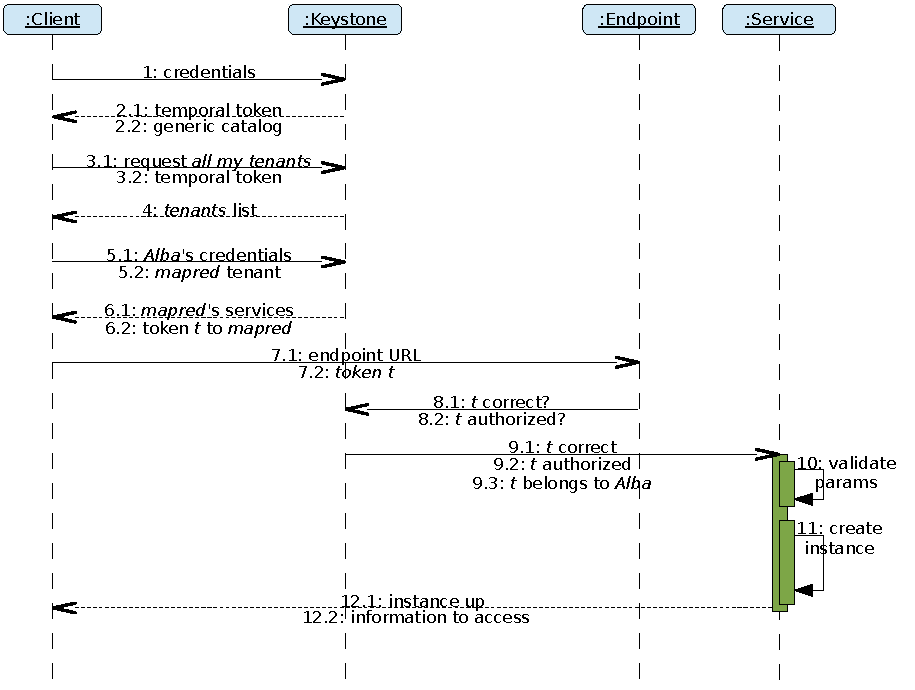
\includegraphics[width=0.99\textwidth]{imagenes/013.pdf}
 \caption{Diagrama de Secuencia --- Crear instancia}
\label{fig:secuenciais}
\end{center}
\end{figure}

Para facilitar el manejo de la seguridad, y ya que Horizon implementa s\'olo un subconjunto de la funcionalidad del cloud, Keystone instala una he\-rra\-mien\-ta CLI para interactuar con el servicio REST que define la ejecuci\'on de las operaciones administrativas. La invocaci\'on por l\'inea de comandos de \'ordenes de gesti\'on requiere conocer el token de administrador (\emph{admin token}), que habr\'a de ser convenientemente protegido, o bien hacer invocaciones con un usuario que posea el rol de ad\-mi\-nis\-tra\-dor. Por \'ultimo, a\~nadir que Keystone utiliza una base de datos para que la informaci\'on de acceso de los usuarios y del cat\'alogo de servicios del cloud sea persistente ---normalmente \texttt{MySQL}, en producci\'on, o \texttt{sqlite}.


\section{Quantum}\label{sec:quantum}
\noindent Quantum es el nuevo m\'odulo en OpenStack Folsom para gestionar el des\-plie\-gue de red virtual. En la versi\'on previa del cloud (Essex) se utilizaba un servicio embebido en el propio m\'odulo Compute (Network), que configuraba la red virtual pero de forma m\'as acoplada. El hecho de que haya aparecido un m\'odulo aislado para mantener la red no es casual, y es que OpenStack evoluciona dando especial \'enfasis a la modularidad de sus servicios. Como funciona de forma totalmente aut\'onoma, se podr\'ia dedicar un servidor al completo para manejar Quantum. Para cubrir su funcionalidad, Quantum se apoya en unos plugins y en otros servicios del anfitri\'on en el que resida.\newline

Dos de los posibles plugins que pueden usarse en despliegues con Quantum son: \texttt{OpenVSwitch} y \texttt{LinuxBridge}. La configuraci\'on de la infraestructura de red virtual, tanto con OpenVSwitch como con LinuxBridge, est\'a cubierta con cierto detalle en el manual del administrador de Quantum para OpenStack Folsom \cite{quantumadminfolsom}. Quantum se vale, adicionalmente, de iptables para con\-fi\-gu\-rar el firewall y el enrutamiento de paqueter\'ia, y de \texttt{dnsmasq} para el \emph{DNS} (\emph{Domain Name Server}), el \emph{DHCP} (\emph{Dynamic Host Configuration Protocol}), y la \emph{NAT} (\emph{Network Address Translation}).\newline

La figura \ref{fig:desplieguequantum} muestra un ejemplo de topolog\'ia de red virtual en el que cada proyecto tiene asignado un router virtual particular. Adem\'as, a cada proyecto se le pueden adjudicar nuevos enrutadores que gestionar\'an las redes virtuales privadas asociadas. El solapamiento de IPs privadas en las subredes de cada router virtual est\'a permitido, como se observa en la figura. La IP p\'ublica (flotante) de cada router y de cada m\'aquina virtual ha de asignarse de la subred de la red externa (\texttt{30.0.0.0/22} en la figura). Por \'ultimo, apuntar que las direcciones de red \texttt{30.0.0.X} se corresponden con IPs p\'ublicas, y las \texttt{10.0.X.Y} con IPs privadas, esto es, no accesibles desde m\'as all\'a de cada router.\newline

\begin{figure}[tbh]
\begin{center}
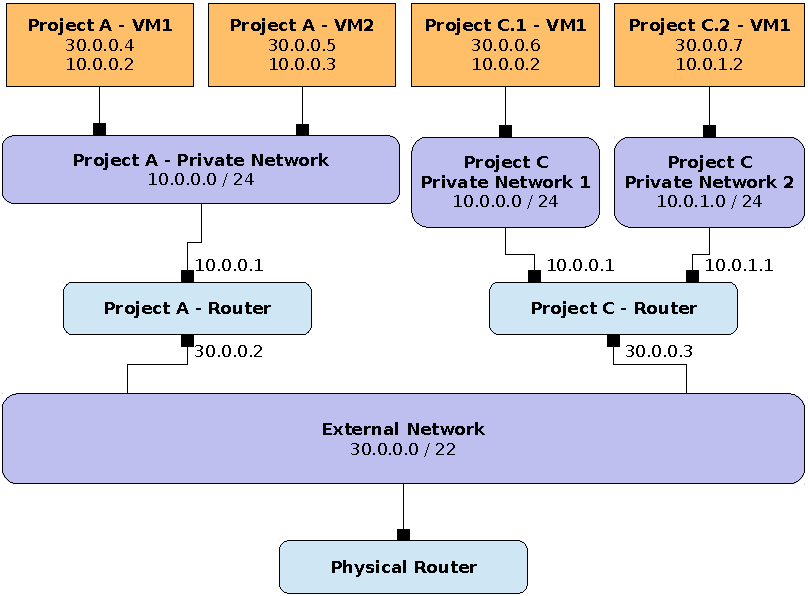
\includegraphics[width=0.9\textwidth]{imagenes/014.pdf}
 \caption{Ejemplo de despliegue avanzado de red virtual con Quantum}
\label{fig:desplieguequantum}
\end{center}
\end{figure}

Este ejemplo representa un despliegue de red virtual de lo m\'as gen\'erico; es posible, no obstante, definir topolog\'ias menos complejas en caso de que no fuese necesaria la aparici\'on de un enrutador en cada proyecto.


\section{Compute}\label{sec:compute}
\noindent Compute es el m\'odulo central de OpenStack. Su cometido consiste en orquestar el funcionamiento global del cloud, delegando cada funci\'on concreta al servicio responsable. A trav\'es de la interacci\'on con el servicio compute, seremos capaces de concebir nuevas instancias de servidores virtuales, que tomar\'an prestados ciclos de CPU, memoria RAM, memoria de disco e interfaces de red, de la capa hardware subyacente. OpenStack Compute no incluye un paquete de virtualizaci\'on hardware. Su aproximaci\'on a esa necesidad consiste en delegar el aprovisionamiento de infraestructuta en alg\'un servicio vir\-tua\-li\-za\-dor al que tenga acceso, ya sea en el mismo nodo donde resida Compute o en otro. Para exponer este servicio de procesado bajo demanda, Compute define, adem\'as, una interfaz en forma de API REST para que los usuarios dirijan el ciclo de vida de las instancias dentro del cloud.\newline

Para poner en marcha una instancia no s\'olo se requiere la colaboraci\'on del hipervisor. Previamente, Compute establecer\'a comunicaciones as\'incronas con el resto de los componentes del cloud para configurar la ejecuci\'on.

\begin{description}
 \item[Keystone:] coteja credenciales y autoriza peticiones.
 \item[Glance:] selecciona la imagen que ha de ser arrancada.
 \item[Quantum:] otorga IPs privadas y p\'ublicas y controla el tr\'afico de red de la instancia.
 \item[Cinder:] maneja el almacenamiento en bloque y el enganche en caliente de vol\'umenes.
 \item[Qpid:] soporta el intercambio de mensajes con los APIs de Keystone, Quantum, Glance y/o Cinder.
\end{description}

Se ha venido diciendo a lo largo del texto que si algo alinea a los distintos cloud es su flexibilidad. Puesto que las necesidades computacionales de los usuarios var\'ian en funci\'on del tiempo, es necesario que, dentro de unos l\'imites, se les permita concretar las caracter\'isticas t\'ecnicas de las m\'aquinas virtuales. En OpenStack cada posible configuraci\'on instanciable, esto es, cada realizaci\'on concreta de la cantidad de recursos que temporalmente se expropian del anfitri\'on, se denomina \emph{flavor} ---siguiendo la nomenclatura de los AWS. De manera que se va a otorgar la posibilidad de que los usuarios autorizados puedan crear sus propios \emph{sabores} computacionales, definiendo el tama\~no del disco, el n\'umero de VCPUs, etc., sin ninguna dificultad, a trav\'es de Horizon.


\section{Glance}\label{sec:glance}
\noindent Glance es el servicio de hospedaje de im\'agenes para OpenStack. Se pueden configurar m\'ultiples backends de datos para guardarlas como: Swift, Amazon S3, el sistema de ficheros local o una ubicaci\'on HTTP; lo que mantiene el nivel de flexibilidad a la par con los dem\'as m\'odulos. Glance se vale de Keystone para manejar el acceso y la seguridad de las im\'agenes y se comunica con Compute para ponerlas en ejecuci\'on bajo demanda.
Ofrece soporte a una buena variedad de clases de im\'agenes y formatos de su contenedor; pero este hecho es meramente informativo para el cloud, ya que la capacidad o incapacidad de arrancar una instancia est\'a vinculada al hipervisor desplegado y no a Glance. Tambi\'en est\'a presente la habilidad de asociar metadatos a las im\'agenes en forma de pares \texttt{(clave, valor)}. Esta metainformaci\'on se utiliza para diferenciar distintas im\'agenes o para configurar el \emph{direct kernel boot} necesario para redimensionar el volumen ra\'iz al arrancar las im\'agenes en distintos sabores.


\section{Almacenamiento}\label{sec:almacenamiento}
\noindent OpenStack otorga tres opciones a la hora de elegir el tipo de almacenamiento:
\begin{description}
 \item[Vol\'atil:] las dimensiones del disco r\'igido sobre el que se dispone la ra\'iz del \'arbol de ficheros se fijan, en el momento de arrancar la m\'aquina virtual, a las marcadas por el sabor elegido. Los archivos contenidos en \'el son aquellos que aparecen en la definici\'on de la imagen del sistema almacenada en Glance. Las alteraciones de este sistema de ficheros no persisten entre ejecuciones de las instancias. Al ordenar la finalizaci\'on de la ejecuci\'on de un servidor virtual, se destruye el fichero temporal que reflejaba las modificaciones del usuario a dicho sistema de ficheros en esa ejecuci\'on concreta.
 \item[Persistente:] vali\'endose de vol\'umenes de almacenamiento gestionados por Cinder con ayuda de \emph{LVM} (\emph{Logical Volume Manager}), OpenStack otorga la posibilidad de enganchar a las instancias, en caliente, vol\'umenes l\'ogicos de tama\~nos indeterminados y creados bajo demanda. Con este tipo de salvaguarda, se garantiza que la informaci\'on no se pierde al terminar la sesi\'on de ejecuci\'on. Sin embargo, este mecanismo de almacenamiento tiene una importante limitaci\'on y es que no es posible enganchar un mismo volumen l\'ogico a dos instancias al mismo tiempo. La alta disponibilidad o la seguridad de la informaci\'on ante fallo no est\'an implementadas directamente, ya que los datos van a residir en un \'unico punto. Podr\'ian superarse estas limitaciones definiendo alguna pol\'itica de copia de seguridad o alguna cofiguraci\'on \emph{RAID} (\emph{Redundant Array of Idependent Disks}) sobre los vol\'umenes ---no recomendable porque OpenStack cuenta con un m\'odulo a tal fin (Swift).
 \item[Seguro:] OpenStack Swift es el m\'odulo que permite la gesti\'on autom\'atica del almacenamiento distribuido de forma segura y permitiendo despliegues para alta disponibilidad. Utiliza la replicaci\'on controlada para establecer el marco de seguridad y la alta disponibilidad, combatiendo as\'i los problemas derivados de la fragilidad inherente a los discos duros. Swift se escuda en \texttt{rsync} para sincronizar las r\'eplicas sobre particiones \emph{XFS}.
\end{description}
 
 
\subsection{Cinder}\label{subsec:cinder}
\noindent Cinder es el m\'odulo de OpenStack que maneja los dispositivos virtuales de almacenamiento en bloque; de funcionalidad similar a la del \emph{EBS} (\emph{Elastic Block Storage}) de Amazon. Cinder utiliza una implementaci\'on de \emph{iSCSI} (\texttt{open-iscsi}) y LVM para Linux para gestionar las operaciones sobre los vol\'umenes. La creaci\'on, el enganche y desacople y el borrado de los bloques de almacenamiento persistente se maneja desde Horizon directamente.\newline

Estos bloques virtuales de persistencia se gestionan como vol\'umenes l\'ogicos pertenecientes a un grupo de vol\'umenes controlado por Cinder. Cinder no pretende crear un medio compartido como \emph{NFS} (\emph{Network File System}), o alguna soluci\'on \emph{SAN} (\emph{Storage Area Network}) o \emph{NAS} (\emph{Network Attached Storage}) para las instancias, ya que no es posible compartir un mismo vo\-lu\-men l\'ogico con m\'as de una m\'aquina virtual en un mismo instante. Una opci\'on interesante, que permite Cinder para facilitar ciertos despligues virtuales heterog\'eneos, es configurar las instancias para que arranquen desde un volumen creado por Cinder.


\subsection{Swift}\label{subsec:swift}
\noindent Al igual que suced\'ia con Cinder, Swift tampoco se enmarca en la idea tradicional de almacenamiento compartido en red, ni debe compararse con el anterior; Cinder y Swift cubren demandas diferentes. Se dice que Swift es ``\textit{un sistema escalable de almacenamiento de objetos, donde los usuarios registrados controlan sus compartimentos de datos o contenedores, subiendo, descargando o borrando ficheros a su antojo}'' \cite{osswift}. Funcionalmente Swift equivale al S3 de Amazon y al \texttt{Walrus} de Eucalyptus, siendo posible con\-fi\-gu\-rar un API REST compatible, parcialmente por el momento (enero 2013), con la sintaxis del primero. Una caracter\'istica fundamental para Swift es la replicaci\'on controlada.


\subsubsection{Replicaci\'on}\label{subsubsec:replicacion}
\noindent La escalabilidad, la tolerancia a fallo, la alta disponibilidad, la seguridad, el balanceo de almacenamiento y el control de carga son algunos de los rasgos que definen a Swift. La alta disponibilidad y la tolerancia a fallo se implementan usando la replicaci\'on. La replicaci\'on es un mecanismo a trav\'es del cual un sistema distribuido mantiene copias o \emph{r\'eplicas} en puntos diferentes de su despliegue, para mejorar sus prestaciones o limitar el alcalce de los fallos, entre otros.\newline

En Swift, los procesos de replicaci\'on de cada \emph{Servidor de Objetos}, que es un nodo cualquiera del cl\'uster con Swift en funcionamiento, van a comparar, peri\'odicamente, sus copias locales con cada copia remota para verificar su grado de actualizaci\'on. Cotejar estas r\'eplicas es un proceso tan costoso computacionalmente como habitual en sistemas de almacenamiento distribuido, por eso Swift se vale de estructuras como las \emph{listas Hash} o las \emph{marcas de agua} para acelerar las comparaciones. Rsync o HTTP gestionan la trans\-fe\-ren\-cia de las copias en funci\'on del tipo de objeto a replicar. La transparencia de replicaci\'on es uno de los pilares que soportan la escalabilidad de Swift. Cuando se a\~nade un nuevo nodo al espacio de almacenamiento de Swift, la redistribuci\'on de las copias es autom\'atica y, desde el momento en que \'este sea sincronizado, podr\'a responder a peticiones de datos de los usuarios.

\subsubsection{Updaters y Auditors}\label{subsubsec:otroscompswift}
\noindent Otros componentes interesantes, que completan el c\'irculo funcional descrito para Swift, son los \emph{Updaters} y los \emph{Auditors}. Los primeros act\'uan cuando se produce un error de sincronizaci\'on entre copias o cuando la carga computacional de un Servidor de Objetos es lo suficientemente alta como para que no pueda satisfacer una operaci\'on. Sucede entonces que la ejecuci\'on de esa operaci\'on se difiere; se a\~nade a una cola de actualizaci\'on que el Updater va procesando para restablecer la sincronizaci\'on. Los Auditors escanean continuamente el sistema de ficheros en busca de fallos de integridad en objetos, contenedores o cuentas de usuario, tal que, si encontrasen incoherencias, pondr\'ian en cuarentena a la entidad y pedir\'ian que se estableciese una nueva r\'eplica.
